% Created by tikzDevice version 0.12.3.1 on 2022-09-05 08:11:22
% !TEX encoding = UTF-8 Unicode
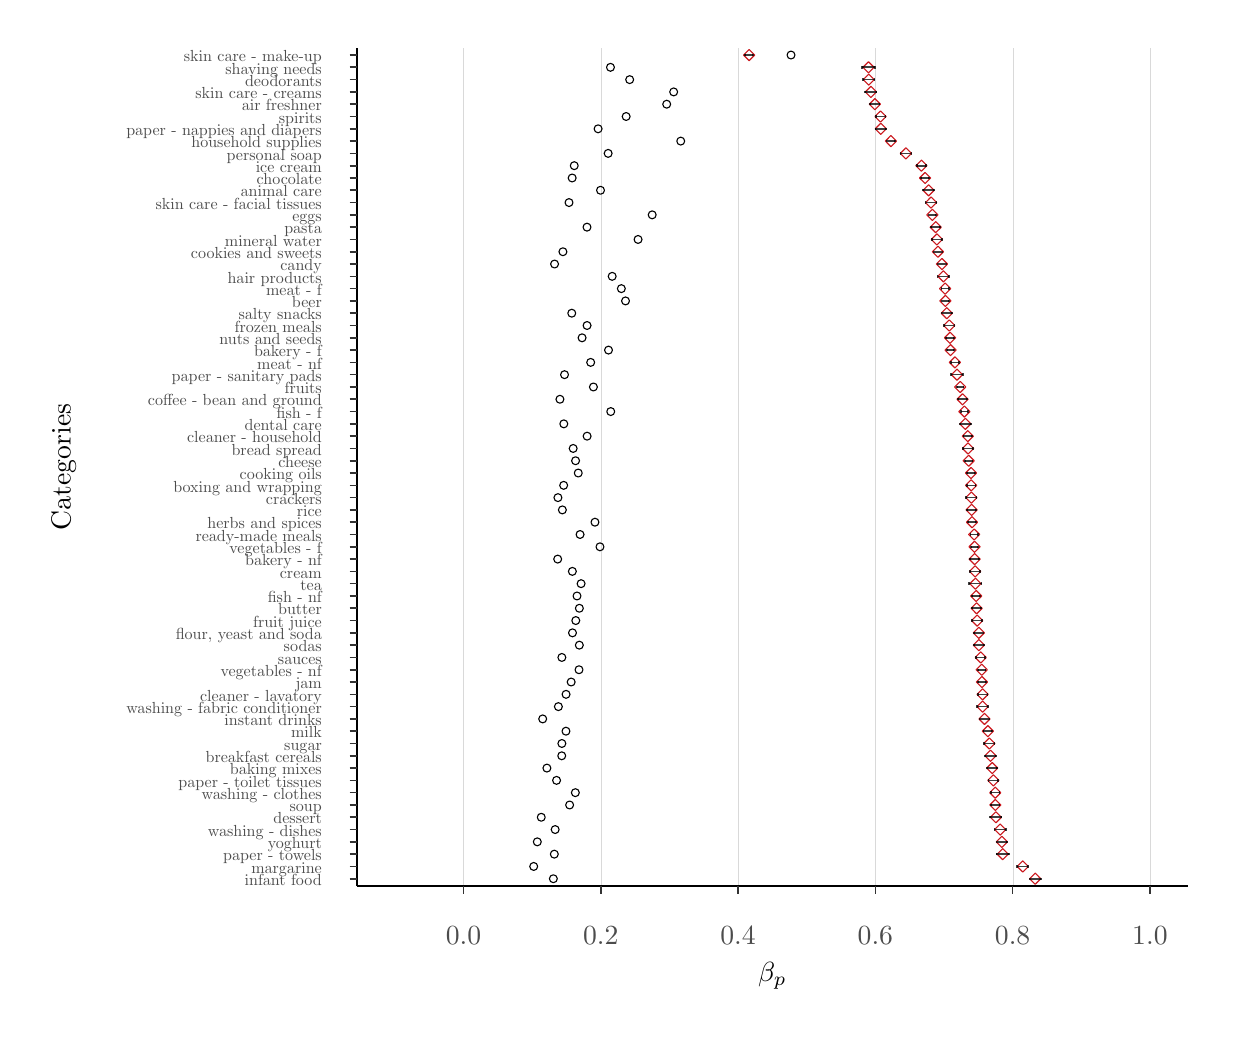
\begin{tikzpicture}[x=1pt,y=1pt]
\definecolor{fillColor}{RGB}{255,255,255}
\path[use as bounding box,fill=fillColor,fill opacity=0.00] (0,0) rectangle (433.62,361.35);
\begin{scope}
\path[clip] (  0.00,  0.00) rectangle (433.62,361.35);
\definecolor{drawColor}{RGB}{255,255,255}
\definecolor{fillColor}{RGB}{255,255,255}

\path[draw=drawColor,line width= 0.6pt,line join=round,line cap=round,fill=fillColor] (  0.00,  0.00) rectangle (433.62,361.35);
\end{scope}
\begin{scope}
\path[clip] (119.04, 51.15) rectangle (419.17,354.12);
\definecolor{drawColor}{RGB}{255,255,255}

\path[draw=drawColor,line width= 0.3pt,line join=round] (132.68, 51.15) --
	(132.68,354.12);

\path[draw=drawColor,line width= 0.3pt,line join=round] (182.29, 51.15) --
	(182.29,354.12);

\path[draw=drawColor,line width= 0.3pt,line join=round] (231.90, 51.15) --
	(231.90,354.12);

\path[draw=drawColor,line width= 0.3pt,line join=round] (281.51, 51.15) --
	(281.51,354.12);

\path[draw=drawColor,line width= 0.3pt,line join=round] (331.11, 51.15) --
	(331.11,354.12);

\path[draw=drawColor,line width= 0.3pt,line join=round] (380.72, 51.15) --
	(380.72,354.12);
\definecolor{drawColor}{gray}{0.85}

\path[draw=drawColor,line width= 0.1pt,line join=round] (157.49, 51.15) --
	(157.49,354.12);

\path[draw=drawColor,line width= 0.1pt,line join=round] (207.09, 51.15) --
	(207.09,354.12);

\path[draw=drawColor,line width= 0.1pt,line join=round] (256.70, 51.15) --
	(256.70,354.12);

\path[draw=drawColor,line width= 0.1pt,line join=round] (306.31, 51.15) --
	(306.31,354.12);

\path[draw=drawColor,line width= 0.1pt,line join=round] (355.92, 51.15) --
	(355.92,354.12);

\path[draw=drawColor,line width= 0.1pt,line join=round] (405.52, 51.15) --
	(405.52,354.12);
\definecolor{drawColor}{RGB}{0,0,0}

\path[draw=drawColor,line width= 0.4pt,line join=round,line cap=round] (230.91,333.69) circle (  1.43);

\path[draw=drawColor,line width= 0.4pt,line join=round,line cap=round] (206.99,302.59) circle (  1.43);

\path[draw=drawColor,line width= 0.4pt,line join=round,line cap=round] (209.88,244.84) circle (  1.43);

\path[draw=drawColor,line width= 0.4pt,line join=round,line cap=round] (191.52,169.32) circle (  1.43);

\path[draw=drawColor,line width= 0.4pt,line join=round,line cap=round] (187.62, 93.80) circle (  1.43);

\path[draw=drawColor,line width= 0.4pt,line join=round,line cap=round] (216.03,262.61) circle (  1.43);

\path[draw=drawColor,line width= 0.4pt,line join=round,line cap=round] (193.68,195.97) circle (  1.43);

\path[draw=drawColor,line width= 0.4pt,line join=round,line cap=round] (197.11,209.30) circle (  1.43);

\path[draw=drawColor,line width= 0.4pt,line join=round,line cap=round] (192.98, 98.24) circle (  1.43);

\path[draw=drawColor,line width= 0.4pt,line join=round,line cap=round] (199.35,151.55) circle (  1.43);

\path[draw=drawColor,line width= 0.4pt,line join=round,line cap=round] (190.39,275.94) circle (  1.43);

\path[draw=drawColor,line width= 0.4pt,line join=round,line cap=round] (197.98,204.86) circle (  1.43);

\path[draw=drawColor,line width= 0.4pt,line join=round,line cap=round] (196.75,307.03) circle (  1.43);

\path[draw=drawColor,line width= 0.4pt,line join=round,line cap=round] (202.15,213.74) circle (  1.43);

\path[draw=drawColor,line width= 0.4pt,line join=round,line cap=round] (194.54,120.45) circle (  1.43);

\path[draw=drawColor,line width= 0.4pt,line join=round,line cap=round] (192.33,227.07) circle (  1.43);

\path[draw=drawColor,line width= 0.4pt,line join=round,line cap=round] (193.41,280.38) circle (  1.43);

\path[draw=drawColor,line width= 0.4pt,line join=round,line cap=round] (198.95,200.42) circle (  1.43);

\path[draw=drawColor,line width= 0.4pt,line join=round,line cap=round] (191.61,191.53) circle (  1.43);

\path[draw=drawColor,line width= 0.4pt,line join=round,line cap=round] (196.82,164.88) circle (  1.43);

\path[draw=drawColor,line width= 0.4pt,line join=round,line cap=round] (193.73,218.19) circle (  1.43);

\path[draw=drawColor,line width= 0.4pt,line join=round,line cap=round] (217.53,342.57) circle (  1.43);

\path[draw=drawColor,line width= 0.4pt,line join=round,line cap=round] (185.58, 76.03) circle (  1.43);

\path[draw=drawColor,line width= 0.4pt,line join=round,line cap=round] (225.67,293.71) circle (  1.43);

\path[draw=drawColor,line width= 0.4pt,line join=round,line cap=round] (210.69,222.63) circle (  1.43);

\path[draw=drawColor,line width= 0.4pt,line join=round,line cap=round] (198.50,155.99) circle (  1.43);

\path[draw=drawColor,line width= 0.4pt,line join=round,line cap=round] (196.87,142.67) circle (  1.43);

\path[draw=drawColor,line width= 0.4pt,line join=round,line cap=round] (202.13,253.73) circle (  1.43);

\path[draw=drawColor,line width= 0.4pt,line join=round,line cap=round] (198.06,147.11) circle (  1.43);

\path[draw=drawColor,line width= 0.4pt,line join=round,line cap=round] (204.43,231.51) circle (  1.43);

\path[draw=drawColor,line width= 0.4pt,line join=round,line cap=round] (211.21,271.49) circle (  1.43);

\path[draw=drawColor,line width= 0.4pt,line join=round,line cap=round] (204.99,182.65) circle (  1.43);

\path[draw=drawColor,line width= 0.4pt,line join=round,line cap=round] (235.98,320.36) circle (  1.43);

\path[draw=drawColor,line width= 0.4pt,line join=round,line cap=round] (197.50,311.48) circle (  1.43);

\path[draw=drawColor,line width= 0.4pt,line join=round,line cap=round] (189.95, 53.82) circle (  1.43);

\path[draw=drawColor,line width= 0.4pt,line join=round,line cap=round] (186.10,111.57) circle (  1.43);

\path[draw=drawColor,line width= 0.4pt,line join=round,line cap=round] (196.39,124.90) circle (  1.43);

\path[draw=drawColor,line width= 0.4pt,line join=round,line cap=round] (182.85, 58.26) circle (  1.43);

\path[draw=drawColor,line width= 0.4pt,line join=round,line cap=round] (214.52,267.05) circle (  1.43);

\path[draw=drawColor,line width= 0.4pt,line join=round,line cap=round] (203.44,240.40) circle (  1.43);

\path[draw=drawColor,line width= 0.4pt,line join=round,line cap=round] (194.51,107.13) circle (  1.43);

\path[draw=drawColor,line width= 0.4pt,line join=round,line cap=round] (220.56,284.82) circle (  1.43);

\path[draw=drawColor,line width= 0.4pt,line join=round,line cap=round] (200.33,249.28) circle (  1.43);

\path[draw=drawColor,line width= 0.4pt,line join=round,line cap=round] (206.12,324.80) circle (  1.43);

\path[draw=drawColor,line width= 0.4pt,line join=round,line cap=round] (193.99,235.96) circle (  1.43);

\path[draw=drawColor,line width= 0.4pt,line join=round,line cap=round] (191.11, 89.36) circle (  1.43);

\path[draw=drawColor,line width= 0.4pt,line join=round,line cap=round] (190.30, 62.70) circle (  1.43);

\path[draw=drawColor,line width= 0.4pt,line join=round,line cap=round] (202.11,289.26) circle (  1.43);

\path[draw=drawColor,line width= 0.4pt,line join=round,line cap=round] (209.75,315.92) circle (  1.43);

\path[draw=drawColor,line width= 0.4pt,line join=round,line cap=round] (199.60,178.21) circle (  1.43);

\path[draw=drawColor,line width= 0.4pt,line join=round,line cap=round] (193.21,187.09) circle (  1.43);

\path[draw=drawColor,line width= 0.4pt,line join=round,line cap=round] (196.60,258.17) circle (  1.43);

\path[draw=drawColor,line width= 0.4pt,line join=round,line cap=round] (193.03,133.78) circle (  1.43);

\path[draw=drawColor,line width= 0.4pt,line join=round,line cap=round] (210.59,347.02) circle (  1.43);

\path[draw=drawColor,line width= 0.4pt,line join=round,line cap=round] (233.43,338.13) circle (  1.43);

\path[draw=drawColor,line width= 0.4pt,line join=round,line cap=round] (195.61,298.15) circle (  1.43);

\path[draw=drawColor,line width= 0.4pt,line join=round,line cap=round] (275.83,351.46) circle (  1.43);

\path[draw=drawColor,line width= 0.4pt,line join=round,line cap=round] (199.34,138.22) circle (  1.43);

\path[draw=drawColor,line width= 0.4pt,line join=round,line cap=round] (195.83, 80.47) circle (  1.43);

\path[draw=drawColor,line width= 0.4pt,line join=round,line cap=round] (216.26,329.25) circle (  1.43);

\path[draw=drawColor,line width= 0.4pt,line join=round,line cap=round] (193.03,102.69) circle (  1.43);

\path[draw=drawColor,line width= 0.4pt,line join=round,line cap=round] (199.97,160.44) circle (  1.43);

\path[draw=drawColor,line width= 0.4pt,line join=round,line cap=round] (206.80,173.76) circle (  1.43);

\path[draw=drawColor,line width= 0.4pt,line join=round,line cap=round] (199.22,129.34) circle (  1.43);

\path[draw=drawColor,line width= 0.4pt,line join=round,line cap=round] (197.90, 84.92) circle (  1.43);

\path[draw=drawColor,line width= 0.4pt,line join=round,line cap=round] (190.60, 71.59) circle (  1.43);

\path[draw=drawColor,line width= 0.4pt,line join=round,line cap=round] (191.77,116.01) circle (  1.43);

\path[draw=drawColor,line width= 0.4pt,line join=round,line cap=round] (184.15, 67.15) circle (  1.43);
\definecolor{drawColor}{RGB}{203,24,29}

\path[draw=drawColor,line width= 0.4pt,line join=round,line cap=round] (304.12,333.69) --
	(306.13,335.71) --
	(308.15,333.69) --
	(306.13,331.67) --
	cycle;

\path[draw=drawColor,line width= 0.4pt,line join=round,line cap=round] (323.54,302.59) --
	(325.56,304.61) --
	(327.58,302.59) --
	(325.56,300.57) --
	cycle;

\path[draw=drawColor,line width= 0.4pt,line join=round,line cap=round] (331.45,244.84) --
	(333.47,246.86) --
	(335.49,244.84) --
	(333.47,242.82) --
	cycle;

\path[draw=drawColor,line width= 0.4pt,line join=round,line cap=round] (340.18,169.32) --
	(342.19,171.34) --
	(344.21,169.32) --
	(342.19,167.30) --
	cycle;

\path[draw=drawColor,line width= 0.4pt,line join=round,line cap=round] (346.53, 93.80) --
	(348.55, 95.82) --
	(350.57, 93.80) --
	(348.55, 91.78) --
	cycle;

\path[draw=drawColor,line width= 0.4pt,line join=round,line cap=round] (329.61,262.61) --
	(331.63,264.63) --
	(333.65,262.61) --
	(331.63,260.59) --
	cycle;

\path[draw=drawColor,line width= 0.4pt,line join=round,line cap=round] (338.91,195.97) --
	(340.93,197.99) --
	(342.95,195.97) --
	(340.93,193.96) --
	cycle;

\path[draw=drawColor,line width= 0.4pt,line join=round,line cap=round] (337.77,209.30) --
	(339.79,211.32) --
	(341.81,209.30) --
	(339.79,207.28) --
	cycle;

\path[draw=drawColor,line width= 0.4pt,line join=round,line cap=round] (345.89, 98.24) --
	(347.91,100.26) --
	(349.93, 98.24) --
	(347.91, 96.23) --
	cycle;

\path[draw=drawColor,line width= 0.4pt,line join=round,line cap=round] (340.89,151.55) --
	(342.90,153.57) --
	(344.92,151.55) --
	(342.90,149.53) --
	cycle;

\path[draw=drawColor,line width= 0.4pt,line join=round,line cap=round] (328.36,275.94) --
	(330.38,277.95) --
	(332.39,275.94) --
	(330.38,273.92) --
	cycle;

\path[draw=drawColor,line width= 0.4pt,line join=round,line cap=round] (338.01,204.86) --
	(340.02,206.88) --
	(342.04,204.86) --
	(340.02,202.84) --
	cycle;

\path[draw=drawColor,line width= 0.4pt,line join=round,line cap=round] (322.26,307.03) --
	(324.28,309.05) --
	(326.29,307.03) --
	(324.28,305.02) --
	cycle;

\path[draw=drawColor,line width= 0.4pt,line join=round,line cap=round] (337.69,213.74) --
	(339.70,215.76) --
	(341.72,213.74) --
	(339.70,211.73) --
	cycle;

\path[draw=drawColor,line width= 0.4pt,line join=round,line cap=round] (343.03,120.45) --
	(345.05,122.47) --
	(347.07,120.45) --
	(345.05,118.44) --
	cycle;

\path[draw=drawColor,line width= 0.4pt,line join=round,line cap=round] (335.81,227.07) --
	(337.82,229.09) --
	(339.84,227.07) --
	(337.82,225.05) --
	cycle;

\path[draw=drawColor,line width= 0.4pt,line join=round,line cap=round] (326.90,280.38) --
	(328.92,282.40) --
	(330.93,280.38) --
	(328.92,278.36) --
	cycle;

\path[draw=drawColor,line width= 0.4pt,line join=round,line cap=round] (338.86,200.42) --
	(340.87,202.43) --
	(342.89,200.42) --
	(340.87,198.40) --
	cycle;

\path[draw=drawColor,line width= 0.4pt,line join=round,line cap=round] (338.98,191.53) --
	(340.99,193.55) --
	(343.01,191.53) --
	(340.99,189.51) --
	cycle;

\path[draw=drawColor,line width= 0.4pt,line join=round,line cap=round] (340.35,164.88) --
	(342.37,166.90) --
	(344.39,164.88) --
	(342.37,162.86) --
	cycle;

\path[draw=drawColor,line width= 0.4pt,line join=round,line cap=round] (336.80,218.19) --
	(338.82,220.20) --
	(340.83,218.19) --
	(338.82,216.17) --
	cycle;

\path[draw=drawColor,line width= 0.4pt,line join=round,line cap=round] (301.90,342.57) --
	(303.92,344.59) --
	(305.93,342.57) --
	(303.92,340.56) --
	cycle;

\path[draw=drawColor,line width= 0.4pt,line join=round,line cap=round] (347.84, 76.03) --
	(349.86, 78.05) --
	(351.88, 76.03) --
	(349.86, 74.01) --
	cycle;

\path[draw=drawColor,line width= 0.4pt,line join=round,line cap=round] (324.89,293.71) --
	(326.90,295.72) --
	(328.92,293.71) --
	(326.90,291.69) --
	cycle;

\path[draw=drawColor,line width= 0.4pt,line join=round,line cap=round] (336.46,222.63) --
	(338.47,224.65) --
	(340.49,222.63) --
	(338.47,220.61) --
	cycle;

\path[draw=drawColor,line width= 0.4pt,line join=round,line cap=round] (340.71,155.99) --
	(342.73,158.01) --
	(344.75,155.99) --
	(342.73,153.98) --
	cycle;

\path[draw=drawColor,line width= 0.4pt,line join=round,line cap=round] (341.68,142.67) --
	(343.70,144.68) --
	(345.72,142.67) --
	(343.70,140.65) --
	cycle;

\path[draw=drawColor,line width= 0.4pt,line join=round,line cap=round] (331.00,253.73) --
	(333.01,255.74) --
	(335.03,253.73) --
	(333.01,251.71) --
	cycle;

\path[draw=drawColor,line width= 0.4pt,line join=round,line cap=round] (341.07,147.11) --
	(343.09,149.13) --
	(345.11,147.11) --
	(343.09,145.09) --
	cycle;

\path[draw=drawColor,line width= 0.4pt,line join=round,line cap=round] (334.94,231.51) --
	(336.96,233.53) --
	(338.98,231.51) --
	(336.96,229.50) --
	cycle;

\path[draw=drawColor,line width= 0.4pt,line join=round,line cap=round] (328.88,271.49) --
	(330.90,273.51) --
	(332.91,271.49) --
	(330.90,269.48) --
	cycle;

\path[draw=drawColor,line width= 0.4pt,line join=round,line cap=round] (339.22,182.65) --
	(341.23,184.67) --
	(343.25,182.65) --
	(341.23,180.63) --
	cycle;

\path[draw=drawColor,line width= 0.4pt,line join=round,line cap=round] (309.93,320.36) --
	(311.94,322.38) --
	(313.96,320.36) --
	(311.94,318.34) --
	cycle;

\path[draw=drawColor,line width= 0.4pt,line join=round,line cap=round] (320.94,311.48) --
	(322.96,313.49) --
	(324.97,311.48) --
	(322.96,309.46) --
	cycle;

\path[draw=drawColor,line width= 0.4pt,line join=round,line cap=round] (362.04, 53.82) --
	(364.06, 55.84) --
	(366.07, 53.82) --
	(364.06, 51.80) --
	cycle;

\path[draw=drawColor,line width= 0.4pt,line join=round,line cap=round] (343.72,111.57) --
	(345.74,113.59) --
	(347.76,111.57) --
	(345.74,109.55) --
	cycle;

\path[draw=drawColor,line width= 0.4pt,line join=round,line cap=round] (342.81,124.90) --
	(344.83,126.91) --
	(346.85,124.90) --
	(344.83,122.88) --
	cycle;

\path[draw=drawColor,line width= 0.4pt,line join=round,line cap=round] (357.55, 58.26) --
	(359.57, 60.28) --
	(361.59, 58.26) --
	(359.57, 56.24) --
	cycle;

\path[draw=drawColor,line width= 0.4pt,line join=round,line cap=round] (329.49,267.05) --
	(331.51,269.07) --
	(333.53,267.05) --
	(331.51,265.04) --
	cycle;

\path[draw=drawColor,line width= 0.4pt,line join=round,line cap=round] (333.05,240.40) --
	(335.07,242.42) --
	(337.08,240.40) --
	(335.07,238.38) --
	cycle;

\path[draw=drawColor,line width= 0.4pt,line join=round,line cap=round] (344.95,107.13) --
	(346.96,109.14) --
	(348.98,107.13) --
	(346.96,105.11) --
	cycle;

\path[draw=drawColor,line width= 0.4pt,line join=round,line cap=round] (326.53,284.82) --
	(328.55,286.84) --
	(330.57,284.82) --
	(328.55,282.80) --
	cycle;

\path[draw=drawColor,line width= 0.4pt,line join=round,line cap=round] (331.27,249.28) --
	(333.29,251.30) --
	(335.31,249.28) --
	(333.29,247.27) --
	cycle;

\path[draw=drawColor,line width= 0.4pt,line join=round,line cap=round] (306.25,324.80) --
	(308.27,326.82) --
	(310.29,324.80) --
	(308.27,322.79) --
	cycle;

\path[draw=drawColor,line width= 0.4pt,line join=round,line cap=round] (333.78,235.96) --
	(335.80,237.97) --
	(337.81,235.96) --
	(335.80,233.94) --
	cycle;

\path[draw=drawColor,line width= 0.4pt,line join=round,line cap=round] (346.94, 89.36) --
	(348.96, 91.38) --
	(350.98, 89.36) --
	(348.96, 87.34) --
	cycle;

\path[draw=drawColor,line width= 0.4pt,line join=round,line cap=round] (350.31, 62.70) --
	(352.33, 64.72) --
	(354.35, 62.70) --
	(352.33, 60.69) --
	cycle;

\path[draw=drawColor,line width= 0.4pt,line join=round,line cap=round] (326.10,289.26) --
	(328.12,291.28) --
	(330.14,289.26) --
	(328.12,287.25) --
	cycle;

\path[draw=drawColor,line width= 0.4pt,line join=round,line cap=round] (315.34,315.92) --
	(317.35,317.94) --
	(319.37,315.92) --
	(317.35,313.90) --
	cycle;

\path[draw=drawColor,line width= 0.4pt,line join=round,line cap=round] (339.99,178.21) --
	(342.00,180.22) --
	(344.02,178.21) --
	(342.00,176.19) --
	cycle;

\path[draw=drawColor,line width= 0.4pt,line join=round,line cap=round] (339.07,187.09) --
	(341.09,189.11) --
	(343.11,187.09) --
	(341.09,185.07) --
	cycle;

\path[draw=drawColor,line width= 0.4pt,line join=round,line cap=round] (330.10,258.17) --
	(332.12,260.19) --
	(334.13,258.17) --
	(332.12,256.15) --
	cycle;

\path[draw=drawColor,line width= 0.4pt,line join=round,line cap=round] (342.38,133.78) --
	(344.40,135.80) --
	(346.41,133.78) --
	(344.40,131.76) --
	cycle;

\path[draw=drawColor,line width= 0.4pt,line join=round,line cap=round] (301.81,347.02) --
	(303.83,349.03) --
	(305.84,347.02) --
	(303.83,345.00) --
	cycle;

\path[draw=drawColor,line width= 0.4pt,line join=round,line cap=round] (302.68,338.13) --
	(304.70,340.15) --
	(306.71,338.13) --
	(304.70,336.11) --
	cycle;

\path[draw=drawColor,line width= 0.4pt,line join=round,line cap=round] (324.42,298.15) --
	(326.43,300.17) --
	(328.45,298.15) --
	(326.43,296.13) --
	cycle;

\path[draw=drawColor,line width= 0.4pt,line join=round,line cap=round] (258.68,351.46) --
	(260.69,353.48) --
	(262.71,351.46) --
	(260.69,349.44) --
	cycle;

\path[draw=drawColor,line width= 0.4pt,line join=round,line cap=round] (341.69,138.22) --
	(343.71,140.24) --
	(345.73,138.22) --
	(343.71,136.21) --
	cycle;

\path[draw=drawColor,line width= 0.4pt,line join=round,line cap=round] (347.65, 80.47) --
	(349.66, 82.49) --
	(351.68, 80.47) --
	(349.66, 78.46) --
	cycle;

\path[draw=drawColor,line width= 0.4pt,line join=round,line cap=round] (306.16,329.25) --
	(308.18,331.26) --
	(310.20,329.25) --
	(308.18,327.23) --
	cycle;

\path[draw=drawColor,line width= 0.4pt,line join=round,line cap=round] (345.47,102.69) --
	(347.49,104.70) --
	(349.50,102.69) --
	(347.49,100.67) --
	cycle;

\path[draw=drawColor,line width= 0.4pt,line join=round,line cap=round] (340.45,160.44) --
	(342.47,162.45) --
	(344.48,160.44) --
	(342.47,158.42) --
	cycle;

\path[draw=drawColor,line width= 0.4pt,line join=round,line cap=round] (340.13,173.76) --
	(342.15,175.78) --
	(344.17,173.76) --
	(342.15,171.75) --
	cycle;

\path[draw=drawColor,line width= 0.4pt,line join=round,line cap=round] (342.72,129.34) --
	(344.74,131.36) --
	(346.76,129.34) --
	(344.74,127.32) --
	cycle;

\path[draw=drawColor,line width= 0.4pt,line join=round,line cap=round] (347.61, 84.92) --
	(349.63, 86.93) --
	(351.64, 84.92) --
	(349.63, 82.90) --
	cycle;

\path[draw=drawColor,line width= 0.4pt,line join=round,line cap=round] (349.39, 71.59) --
	(351.41, 73.61) --
	(353.42, 71.59) --
	(351.41, 69.57) --
	cycle;

\path[draw=drawColor,line width= 0.4pt,line join=round,line cap=round] (343.07,116.01) --
	(345.08,118.03) --
	(347.10,116.01) --
	(345.08,113.99) --
	cycle;

\path[draw=drawColor,line width= 0.4pt,line join=round,line cap=round] (350.01, 67.15) --
	(352.03, 69.16) --
	(354.05, 67.15) --
	(352.03, 65.13) --
	cycle;
\definecolor{drawColor}{RGB}{0,0,0}

\path[draw=drawColor,draw opacity=0.75,line width= 0.6pt,line join=round] (307.83,333.24) --
	(307.83,334.13);

\path[draw=drawColor,draw opacity=0.75,line width= 0.6pt,line join=round] (307.83,333.69) --
	(304.44,333.69);

\path[draw=drawColor,draw opacity=0.75,line width= 0.6pt,line join=round] (304.44,333.24) --
	(304.44,334.13);

\path[draw=drawColor,draw opacity=0.75,line width= 0.6pt,line join=round] (327.51,302.15) --
	(327.51,303.04);

\path[draw=drawColor,draw opacity=0.75,line width= 0.6pt,line join=round] (327.51,302.59) --
	(323.61,302.59);

\path[draw=drawColor,draw opacity=0.75,line width= 0.6pt,line join=round] (323.61,302.15) --
	(323.61,303.04);

\path[draw=drawColor,draw opacity=0.75,line width= 0.6pt,line join=round] (334.71,244.40) --
	(334.71,245.29);

\path[draw=drawColor,draw opacity=0.75,line width= 0.6pt,line join=round] (334.71,244.84) --
	(332.23,244.84);

\path[draw=drawColor,draw opacity=0.75,line width= 0.6pt,line join=round] (332.23,244.40) --
	(332.23,245.29);

\path[draw=drawColor,draw opacity=0.75,line width= 0.6pt,line join=round] (343.80,168.88) --
	(343.80,169.76);

\path[draw=drawColor,draw opacity=0.75,line width= 0.6pt,line join=round] (343.80,169.32) --
	(340.59,169.32);

\path[draw=drawColor,draw opacity=0.75,line width= 0.6pt,line join=round] (340.59,168.88) --
	(340.59,169.76);

\path[draw=drawColor,draw opacity=0.75,line width= 0.6pt,line join=round] (350.38, 93.36) --
	(350.38, 94.24);

\path[draw=drawColor,draw opacity=0.75,line width= 0.6pt,line join=round] (350.38, 93.80) --
	(346.72, 93.80);

\path[draw=drawColor,draw opacity=0.75,line width= 0.6pt,line join=round] (346.72, 93.36) --
	(346.72, 94.24);

\path[draw=drawColor,draw opacity=0.75,line width= 0.6pt,line join=round] (333.03,262.17) --
	(333.03,263.05);

\path[draw=drawColor,draw opacity=0.75,line width= 0.6pt,line join=round] (333.03,262.61) --
	(330.23,262.61);

\path[draw=drawColor,draw opacity=0.75,line width= 0.6pt,line join=round] (330.23,262.17) --
	(330.23,263.05);

\path[draw=drawColor,draw opacity=0.75,line width= 0.6pt,line join=round] (342.53,195.53) --
	(342.53,196.42);

\path[draw=drawColor,draw opacity=0.75,line width= 0.6pt,line join=round] (342.53,195.97) --
	(339.33,195.97);

\path[draw=drawColor,draw opacity=0.75,line width= 0.6pt,line join=round] (339.33,195.53) --
	(339.33,196.42);

\path[draw=drawColor,draw opacity=0.75,line width= 0.6pt,line join=round] (341.57,208.86) --
	(341.57,209.75);

\path[draw=drawColor,draw opacity=0.75,line width= 0.6pt,line join=round] (341.57,209.30) --
	(338.02,209.30);

\path[draw=drawColor,draw opacity=0.75,line width= 0.6pt,line join=round] (338.02,208.86) --
	(338.02,209.75);

\path[draw=drawColor,draw opacity=0.75,line width= 0.6pt,line join=round] (349.82, 97.80) --
	(349.82, 98.69);

\path[draw=drawColor,draw opacity=0.75,line width= 0.6pt,line join=round] (349.82, 98.24) --
	(346.00, 98.24);

\path[draw=drawColor,draw opacity=0.75,line width= 0.6pt,line join=round] (346.00, 97.80) --
	(346.00, 98.69);

\path[draw=drawColor,draw opacity=0.75,line width= 0.6pt,line join=round] (344.52,151.11) --
	(344.52,152.00);

\path[draw=drawColor,draw opacity=0.75,line width= 0.6pt,line join=round] (344.52,151.55) --
	(341.28,151.55);

\path[draw=drawColor,draw opacity=0.75,line width= 0.6pt,line join=round] (341.28,151.11) --
	(341.28,152.00);

\path[draw=drawColor,draw opacity=0.75,line width= 0.6pt,line join=round] (331.97,275.49) --
	(331.97,276.38);

\path[draw=drawColor,draw opacity=0.75,line width= 0.6pt,line join=round] (331.97,275.94) --
	(328.78,275.94);

\path[draw=drawColor,draw opacity=0.75,line width= 0.6pt,line join=round] (328.78,275.49) --
	(328.78,276.38);

\path[draw=drawColor,draw opacity=0.75,line width= 0.6pt,line join=round] (341.44,204.42) --
	(341.44,205.30);

\path[draw=drawColor,draw opacity=0.75,line width= 0.6pt,line join=round] (341.44,204.86) --
	(338.61,204.86);

\path[draw=drawColor,draw opacity=0.75,line width= 0.6pt,line join=round] (338.61,204.42) --
	(338.61,205.30);

\path[draw=drawColor,draw opacity=0.75,line width= 0.6pt,line join=round] (325.76,306.59) --
	(325.76,307.48);

\path[draw=drawColor,draw opacity=0.75,line width= 0.6pt,line join=round] (325.76,307.03) --
	(322.79,307.03);

\path[draw=drawColor,draw opacity=0.75,line width= 0.6pt,line join=round] (322.79,306.59) --
	(322.79,307.48);

\path[draw=drawColor,draw opacity=0.75,line width= 0.6pt,line join=round] (341.30,213.30) --
	(341.30,214.19);

\path[draw=drawColor,draw opacity=0.75,line width= 0.6pt,line join=round] (341.30,213.74) --
	(338.10,213.74);

\path[draw=drawColor,draw opacity=0.75,line width= 0.6pt,line join=round] (338.10,213.30) --
	(338.10,214.19);

\path[draw=drawColor,draw opacity=0.75,line width= 0.6pt,line join=round] (346.81,120.01) --
	(346.81,120.90);

\path[draw=drawColor,draw opacity=0.75,line width= 0.6pt,line join=round] (346.81,120.45) --
	(343.29,120.45);

\path[draw=drawColor,draw opacity=0.75,line width= 0.6pt,line join=round] (343.29,120.01) --
	(343.29,120.90);

\path[draw=drawColor,draw opacity=0.75,line width= 0.6pt,line join=round] (339.42,226.63) --
	(339.42,227.52);

\path[draw=drawColor,draw opacity=0.75,line width= 0.6pt,line join=round] (339.42,227.07) --
	(336.23,227.07);

\path[draw=drawColor,draw opacity=0.75,line width= 0.6pt,line join=round] (336.23,226.63) --
	(336.23,227.52);

\path[draw=drawColor,draw opacity=0.75,line width= 0.6pt,line join=round] (330.52,279.94) --
	(330.52,280.82);

\path[draw=drawColor,draw opacity=0.75,line width= 0.6pt,line join=round] (330.52,280.38) --
	(327.32,280.38);

\path[draw=drawColor,draw opacity=0.75,line width= 0.6pt,line join=round] (327.32,279.94) --
	(327.32,280.82);

\path[draw=drawColor,draw opacity=0.75,line width= 0.6pt,line join=round] (342.25,199.97) --
	(342.25,200.86);

\path[draw=drawColor,draw opacity=0.75,line width= 0.6pt,line join=round] (342.25,200.42) --
	(339.49,200.42);

\path[draw=drawColor,draw opacity=0.75,line width= 0.6pt,line join=round] (339.49,199.97) --
	(339.49,200.86);

\path[draw=drawColor,draw opacity=0.75,line width= 0.6pt,line join=round] (342.89,191.09) --
	(342.89,191.98);

\path[draw=drawColor,draw opacity=0.75,line width= 0.6pt,line join=round] (342.89,191.53) --
	(339.10,191.53);

\path[draw=drawColor,draw opacity=0.75,line width= 0.6pt,line join=round] (339.10,191.09) --
	(339.10,191.98);

\path[draw=drawColor,draw opacity=0.75,line width= 0.6pt,line join=round] (344.16,164.43) --
	(344.16,165.32);

\path[draw=drawColor,draw opacity=0.75,line width= 0.6pt,line join=round] (344.16,164.88) --
	(340.58,164.88);

\path[draw=drawColor,draw opacity=0.75,line width= 0.6pt,line join=round] (340.58,164.43) --
	(340.58,165.32);

\path[draw=drawColor,draw opacity=0.75,line width= 0.6pt,line join=round] (340.84,217.74) --
	(340.84,218.63);

\path[draw=drawColor,draw opacity=0.75,line width= 0.6pt,line join=round] (340.84,218.19) --
	(336.79,218.19);

\path[draw=drawColor,draw opacity=0.75,line width= 0.6pt,line join=round] (336.79,217.74) --
	(336.79,218.63);

\path[draw=drawColor,draw opacity=0.75,line width= 0.6pt,line join=round] (306.00,342.13) --
	(306.00,343.02);

\path[draw=drawColor,draw opacity=0.75,line width= 0.6pt,line join=round] (306.00,342.57) --
	(301.83,342.57);

\path[draw=drawColor,draw opacity=0.75,line width= 0.6pt,line join=round] (301.83,342.13) --
	(301.83,343.02);

\path[draw=drawColor,draw opacity=0.75,line width= 0.6pt,line join=round] (351.93, 75.59) --
	(351.93, 76.48);

\path[draw=drawColor,draw opacity=0.75,line width= 0.6pt,line join=round] (351.93, 76.03) --
	(347.79, 76.03);

\path[draw=drawColor,draw opacity=0.75,line width= 0.6pt,line join=round] (347.79, 75.59) --
	(347.79, 76.48);

\path[draw=drawColor,draw opacity=0.75,line width= 0.6pt,line join=round] (328.24,293.26) --
	(328.24,294.15);

\path[draw=drawColor,draw opacity=0.75,line width= 0.6pt,line join=round] (328.24,293.71) --
	(325.57,293.71);

\path[draw=drawColor,draw opacity=0.75,line width= 0.6pt,line join=round] (325.57,293.26) --
	(325.57,294.15);

\path[draw=drawColor,draw opacity=0.75,line width= 0.6pt,line join=round] (339.69,222.18) --
	(339.69,223.07);

\path[draw=drawColor,draw opacity=0.75,line width= 0.6pt,line join=round] (339.69,222.63) --
	(337.26,222.63);

\path[draw=drawColor,draw opacity=0.75,line width= 0.6pt,line join=round] (337.26,222.18) --
	(337.26,223.07);

\path[draw=drawColor,draw opacity=0.75,line width= 0.6pt,line join=round] (344.20,155.55) --
	(344.20,156.44);

\path[draw=drawColor,draw opacity=0.75,line width= 0.6pt,line join=round] (344.20,155.99) --
	(341.26,155.99);

\path[draw=drawColor,draw opacity=0.75,line width= 0.6pt,line join=round] (341.26,155.55) --
	(341.26,156.44);

\path[draw=drawColor,draw opacity=0.75,line width= 0.6pt,line join=round] (345.36,142.22) --
	(345.36,143.11);

\path[draw=drawColor,draw opacity=0.75,line width= 0.6pt,line join=round] (345.36,142.67) --
	(342.03,142.67);

\path[draw=drawColor,draw opacity=0.75,line width= 0.6pt,line join=round] (342.03,142.22) --
	(342.03,143.11);

\path[draw=drawColor,draw opacity=0.75,line width= 0.6pt,line join=round] (334.90,253.28) --
	(334.90,254.17);

\path[draw=drawColor,draw opacity=0.75,line width= 0.6pt,line join=round] (334.90,253.73) --
	(331.13,253.73);

\path[draw=drawColor,draw opacity=0.75,line width= 0.6pt,line join=round] (331.13,253.28) --
	(331.13,254.17);

\path[draw=drawColor,draw opacity=0.75,line width= 0.6pt,line join=round] (344.84,146.66) --
	(344.84,147.55);

\path[draw=drawColor,draw opacity=0.75,line width= 0.6pt,line join=round] (344.84,147.11) --
	(341.34,147.11);

\path[draw=drawColor,draw opacity=0.75,line width= 0.6pt,line join=round] (341.34,146.66) --
	(341.34,147.55);

\path[draw=drawColor,draw opacity=0.75,line width= 0.6pt,line join=round] (338.18,231.07) --
	(338.18,231.96);

\path[draw=drawColor,draw opacity=0.75,line width= 0.6pt,line join=round] (338.18,231.51) --
	(335.73,231.51);

\path[draw=drawColor,draw opacity=0.75,line width= 0.6pt,line join=round] (335.73,231.07) --
	(335.73,231.96);

\path[draw=drawColor,draw opacity=0.75,line width= 0.6pt,line join=round] (332.98,271.05) --
	(332.98,271.94);

\path[draw=drawColor,draw opacity=0.75,line width= 0.6pt,line join=round] (332.98,271.49) --
	(328.82,271.49);

\path[draw=drawColor,draw opacity=0.75,line width= 0.6pt,line join=round] (328.82,271.05) --
	(328.82,271.94);

\path[draw=drawColor,draw opacity=0.75,line width= 0.6pt,line join=round] (342.64,182.20) --
	(342.64,183.09);

\path[draw=drawColor,draw opacity=0.75,line width= 0.6pt,line join=round] (342.64,182.65) --
	(339.83,182.65);

\path[draw=drawColor,draw opacity=0.75,line width= 0.6pt,line join=round] (339.83,182.20) --
	(339.83,183.09);

\path[draw=drawColor,draw opacity=0.75,line width= 0.6pt,line join=round] (313.49,319.92) --
	(313.49,320.81);

\path[draw=drawColor,draw opacity=0.75,line width= 0.6pt,line join=round] (313.49,320.36) --
	(310.39,320.36);

\path[draw=drawColor,draw opacity=0.75,line width= 0.6pt,line join=round] (310.39,319.92) --
	(310.39,320.81);

\path[draw=drawColor,draw opacity=0.75,line width= 0.6pt,line join=round] (324.51,311.03) --
	(324.51,311.92);

\path[draw=drawColor,draw opacity=0.75,line width= 0.6pt,line join=round] (324.51,311.48) --
	(321.41,311.48);

\path[draw=drawColor,draw opacity=0.75,line width= 0.6pt,line join=round] (321.41,311.03) --
	(321.41,311.92);

\path[draw=drawColor,draw opacity=0.75,line width= 0.6pt,line join=round] (366.08, 53.37) --
	(366.08, 54.26);

\path[draw=drawColor,draw opacity=0.75,line width= 0.6pt,line join=round] (366.08, 53.82) --
	(362.03, 53.82);

\path[draw=drawColor,draw opacity=0.75,line width= 0.6pt,line join=round] (362.03, 53.37) --
	(362.03, 54.26);

\path[draw=drawColor,draw opacity=0.75,line width= 0.6pt,line join=round] (347.50,111.13) --
	(347.50,112.01);

\path[draw=drawColor,draw opacity=0.75,line width= 0.6pt,line join=round] (347.50,111.57) --
	(343.99,111.57);

\path[draw=drawColor,draw opacity=0.75,line width= 0.6pt,line join=round] (343.99,111.13) --
	(343.99,112.01);

\path[draw=drawColor,draw opacity=0.75,line width= 0.6pt,line join=round] (346.38,124.45) --
	(346.38,125.34);

\path[draw=drawColor,draw opacity=0.75,line width= 0.6pt,line join=round] (346.38,124.90) --
	(343.28,124.90);

\path[draw=drawColor,draw opacity=0.75,line width= 0.6pt,line join=round] (343.28,124.45) --
	(343.28,125.34);

\path[draw=drawColor,draw opacity=0.75,line width= 0.6pt,line join=round] (361.57, 57.82) --
	(361.57, 58.71);

\path[draw=drawColor,draw opacity=0.75,line width= 0.6pt,line join=round] (361.57, 58.26) --
	(357.56, 58.26);

\path[draw=drawColor,draw opacity=0.75,line width= 0.6pt,line join=round] (357.56, 57.82) --
	(357.56, 58.71);

\path[draw=drawColor,draw opacity=0.75,line width= 0.6pt,line join=round] (332.84,266.61) --
	(332.84,267.50);

\path[draw=drawColor,draw opacity=0.75,line width= 0.6pt,line join=round] (332.84,267.05) --
	(330.18,267.05);

\path[draw=drawColor,draw opacity=0.75,line width= 0.6pt,line join=round] (330.18,266.61) --
	(330.18,267.50);

\path[draw=drawColor,draw opacity=0.75,line width= 0.6pt,line join=round] (336.47,239.95) --
	(336.47,240.84);

\path[draw=drawColor,draw opacity=0.75,line width= 0.6pt,line join=round] (336.47,240.40) --
	(333.66,240.40);

\path[draw=drawColor,draw opacity=0.75,line width= 0.6pt,line join=round] (333.66,239.95) --
	(333.66,240.84);

\path[draw=drawColor,draw opacity=0.75,line width= 0.6pt,line join=round] (348.57,106.68) --
	(348.57,107.57);

\path[draw=drawColor,draw opacity=0.75,line width= 0.6pt,line join=round] (348.57,107.13) --
	(345.35,107.13);

\path[draw=drawColor,draw opacity=0.75,line width= 0.6pt,line join=round] (345.35,106.68) --
	(345.35,107.57);

\path[draw=drawColor,draw opacity=0.75,line width= 0.6pt,line join=round] (330.37,284.38) --
	(330.37,285.27);

\path[draw=drawColor,draw opacity=0.75,line width= 0.6pt,line join=round] (330.37,284.82) --
	(326.72,284.82);

\path[draw=drawColor,draw opacity=0.75,line width= 0.6pt,line join=round] (326.72,284.38) --
	(326.72,285.27);

\path[draw=drawColor,draw opacity=0.75,line width= 0.6pt,line join=round] (334.67,248.84) --
	(334.67,249.73);

\path[draw=drawColor,draw opacity=0.75,line width= 0.6pt,line join=round] (334.67,249.28) --
	(331.91,249.28);

\path[draw=drawColor,draw opacity=0.75,line width= 0.6pt,line join=round] (331.91,248.84) --
	(331.91,249.73);

\path[draw=drawColor,draw opacity=0.75,line width= 0.6pt,line join=round] (310.20,324.36) --
	(310.20,325.25);

\path[draw=drawColor,draw opacity=0.75,line width= 0.6pt,line join=round] (310.20,324.80) --
	(306.34,324.80);

\path[draw=drawColor,draw opacity=0.75,line width= 0.6pt,line join=round] (306.34,324.36) --
	(306.34,325.25);

\path[draw=drawColor,draw opacity=0.75,line width= 0.6pt,line join=round] (338.01,235.51) --
	(338.01,236.40);

\path[draw=drawColor,draw opacity=0.75,line width= 0.6pt,line join=round] (338.01,235.96) --
	(333.58,235.96);

\path[draw=drawColor,draw opacity=0.75,line width= 0.6pt,line join=round] (333.58,235.51) --
	(333.58,236.40);

\path[draw=drawColor,draw opacity=0.75,line width= 0.6pt,line join=round] (350.67, 88.91) --
	(350.67, 89.80);

\path[draw=drawColor,draw opacity=0.75,line width= 0.6pt,line join=round] (350.67, 89.36) --
	(347.25, 89.36);

\path[draw=drawColor,draw opacity=0.75,line width= 0.6pt,line join=round] (347.25, 88.91) --
	(347.25, 89.80);

\path[draw=drawColor,draw opacity=0.75,line width= 0.6pt,line join=round] (354.61, 62.26) --
	(354.61, 63.15);

\path[draw=drawColor,draw opacity=0.75,line width= 0.6pt,line join=round] (354.61, 62.70) --
	(350.05, 62.70);

\path[draw=drawColor,draw opacity=0.75,line width= 0.6pt,line join=round] (350.05, 62.26) --
	(350.05, 63.15);

\path[draw=drawColor,draw opacity=0.75,line width= 0.6pt,line join=round] (329.77,288.82) --
	(329.77,289.71);

\path[draw=drawColor,draw opacity=0.75,line width= 0.6pt,line join=round] (329.77,289.26) --
	(326.47,289.26);

\path[draw=drawColor,draw opacity=0.75,line width= 0.6pt,line join=round] (326.47,288.82) --
	(326.47,289.71);

\path[draw=drawColor,draw opacity=0.75,line width= 0.6pt,line join=round] (319.35,315.47) --
	(319.35,316.36);

\path[draw=drawColor,draw opacity=0.75,line width= 0.6pt,line join=round] (319.35,315.92) --
	(315.36,315.92);

\path[draw=drawColor,draw opacity=0.75,line width= 0.6pt,line join=round] (315.36,315.47) --
	(315.36,316.36);

\path[draw=drawColor,draw opacity=0.75,line width= 0.6pt,line join=round] (343.35,177.76) --
	(343.35,178.65);

\path[draw=drawColor,draw opacity=0.75,line width= 0.6pt,line join=round] (343.35,178.21) --
	(340.66,178.21);

\path[draw=drawColor,draw opacity=0.75,line width= 0.6pt,line join=round] (340.66,177.76) --
	(340.66,178.65);

\path[draw=drawColor,draw opacity=0.75,line width= 0.6pt,line join=round] (342.68,186.65) --
	(342.68,187.53);

\path[draw=drawColor,draw opacity=0.75,line width= 0.6pt,line join=round] (342.68,187.09) --
	(339.50,187.09);

\path[draw=drawColor,draw opacity=0.75,line width= 0.6pt,line join=round] (339.50,186.65) --
	(339.50,187.53);

\path[draw=drawColor,draw opacity=0.75,line width= 0.6pt,line join=round] (333.98,257.72) --
	(333.98,258.61);

\path[draw=drawColor,draw opacity=0.75,line width= 0.6pt,line join=round] (333.98,258.17) --
	(330.25,258.17);

\path[draw=drawColor,draw opacity=0.75,line width= 0.6pt,line join=round] (330.25,257.72) --
	(330.25,258.61);

\path[draw=drawColor,draw opacity=0.75,line width= 0.6pt,line join=round] (346.01,133.34) --
	(346.01,134.23);

\path[draw=drawColor,draw opacity=0.75,line width= 0.6pt,line join=round] (346.01,133.78) --
	(342.78,133.78);

\path[draw=drawColor,draw opacity=0.75,line width= 0.6pt,line join=round] (342.78,133.34) --
	(342.78,134.23);

\path[draw=drawColor,draw opacity=0.75,line width= 0.6pt,line join=round] (306.08,346.57) --
	(306.08,347.46);

\path[draw=drawColor,draw opacity=0.75,line width= 0.6pt,line join=round] (306.08,347.02) --
	(301.57,347.02);

\path[draw=drawColor,draw opacity=0.75,line width= 0.6pt,line join=round] (301.57,346.57) --
	(301.57,347.46);

\path[draw=drawColor,draw opacity=0.75,line width= 0.6pt,line join=round] (306.76,337.69) --
	(306.76,338.57);

\path[draw=drawColor,draw opacity=0.75,line width= 0.6pt,line join=round] (306.76,338.13) --
	(302.63,338.13);

\path[draw=drawColor,draw opacity=0.75,line width= 0.6pt,line join=round] (302.63,337.69) --
	(302.63,338.57);

\path[draw=drawColor,draw opacity=0.75,line width= 0.6pt,line join=round] (328.42,297.70) --
	(328.42,298.59);

\path[draw=drawColor,draw opacity=0.75,line width= 0.6pt,line join=round] (328.42,298.15) --
	(324.44,298.15);

\path[draw=drawColor,draw opacity=0.75,line width= 0.6pt,line join=round] (324.44,297.70) --
	(324.44,298.59);

\path[draw=drawColor,draw opacity=0.75,line width= 0.6pt,line join=round] (262.20,351.01) --
	(262.20,351.90);

\path[draw=drawColor,draw opacity=0.75,line width= 0.6pt,line join=round] (262.20,351.46) --
	(259.19,351.46);

\path[draw=drawColor,draw opacity=0.75,line width= 0.6pt,line join=round] (259.19,351.01) --
	(259.19,351.90);

\path[draw=drawColor,draw opacity=0.75,line width= 0.6pt,line join=round] (345.46,137.78) --
	(345.46,138.67);

\path[draw=drawColor,draw opacity=0.75,line width= 0.6pt,line join=round] (345.46,138.22) --
	(341.96,138.22);

\path[draw=drawColor,draw opacity=0.75,line width= 0.6pt,line join=round] (341.96,137.78) --
	(341.96,138.67);

\path[draw=drawColor,draw opacity=0.75,line width= 0.6pt,line join=round] (351.22, 80.03) --
	(351.22, 80.92);

\path[draw=drawColor,draw opacity=0.75,line width= 0.6pt,line join=round] (351.22, 80.47) --
	(348.11, 80.47);

\path[draw=drawColor,draw opacity=0.75,line width= 0.6pt,line join=round] (348.11, 80.03) --
	(348.11, 80.92);

\path[draw=drawColor,draw opacity=0.75,line width= 0.6pt,line join=round] (309.91,328.80) --
	(309.91,329.69);

\path[draw=drawColor,draw opacity=0.75,line width= 0.6pt,line join=round] (309.91,329.25) --
	(306.45,329.25);

\path[draw=drawColor,draw opacity=0.75,line width= 0.6pt,line join=round] (306.45,328.80) --
	(306.45,329.69);

\path[draw=drawColor,draw opacity=0.75,line width= 0.6pt,line join=round] (349.40,102.24) --
	(349.40,103.13);

\path[draw=drawColor,draw opacity=0.75,line width= 0.6pt,line join=round] (349.40,102.69) --
	(345.57,102.69);

\path[draw=drawColor,draw opacity=0.75,line width= 0.6pt,line join=round] (345.57,102.24) --
	(345.57,103.13);

\path[draw=drawColor,draw opacity=0.75,line width= 0.6pt,line join=round] (344.69,159.99) --
	(344.69,160.88);

\path[draw=drawColor,draw opacity=0.75,line width= 0.6pt,line join=round] (344.69,160.44) --
	(340.24,160.44);

\path[draw=drawColor,draw opacity=0.75,line width= 0.6pt,line join=round] (340.24,159.99) --
	(340.24,160.88);

\path[draw=drawColor,draw opacity=0.75,line width= 0.6pt,line join=round] (343.35,173.32) --
	(343.35,174.21);

\path[draw=drawColor,draw opacity=0.75,line width= 0.6pt,line join=round] (343.35,173.76) --
	(340.95,173.76);

\path[draw=drawColor,draw opacity=0.75,line width= 0.6pt,line join=round] (340.95,173.32) --
	(340.95,174.21);

\path[draw=drawColor,draw opacity=0.75,line width= 0.6pt,line join=round] (346.11,128.90) --
	(346.11,129.78);

\path[draw=drawColor,draw opacity=0.75,line width= 0.6pt,line join=round] (346.11,129.34) --
	(343.36,129.34);

\path[draw=drawColor,draw opacity=0.75,line width= 0.6pt,line join=round] (343.36,128.90) --
	(343.36,129.78);

\path[draw=drawColor,draw opacity=0.75,line width= 0.6pt,line join=round] (351.21, 84.47) --
	(351.21, 85.36);

\path[draw=drawColor,draw opacity=0.75,line width= 0.6pt,line join=round] (351.21, 84.92) --
	(348.05, 84.92);

\path[draw=drawColor,draw opacity=0.75,line width= 0.6pt,line join=round] (348.05, 84.47) --
	(348.05, 85.36);

\path[draw=drawColor,draw opacity=0.75,line width= 0.6pt,line join=round] (353.45, 71.14) --
	(353.45, 72.03);

\path[draw=drawColor,draw opacity=0.75,line width= 0.6pt,line join=round] (353.45, 71.59) --
	(349.36, 71.59);

\path[draw=drawColor,draw opacity=0.75,line width= 0.6pt,line join=round] (349.36, 71.14) --
	(349.36, 72.03);

\path[draw=drawColor,draw opacity=0.75,line width= 0.6pt,line join=round] (347.06,115.57) --
	(347.06,116.46);

\path[draw=drawColor,draw opacity=0.75,line width= 0.6pt,line join=round] (347.06,116.01) --
	(343.11,116.01);

\path[draw=drawColor,draw opacity=0.75,line width= 0.6pt,line join=round] (343.11,115.57) --
	(343.11,116.46);

\path[draw=drawColor,draw opacity=0.75,line width= 0.6pt,line join=round] (353.92, 66.70) --
	(353.92, 67.59);

\path[draw=drawColor,draw opacity=0.75,line width= 0.6pt,line join=round] (353.92, 67.15) --
	(350.13, 67.15);

\path[draw=drawColor,draw opacity=0.75,line width= 0.6pt,line join=round] (350.13, 66.70) --
	(350.13, 67.59);
\end{scope}
\begin{scope}
\path[clip] (  0.00,  0.00) rectangle (433.62,361.35);
\definecolor{drawColor}{RGB}{0,0,0}

\path[draw=drawColor,line width= 0.6pt,line join=round] (119.04, 51.15) --
	(119.04,354.12);
\end{scope}
\begin{scope}
\path[clip] (  0.00,  0.00) rectangle (433.62,361.35);
\definecolor{drawColor}{gray}{0.30}

\node[text=drawColor,anchor=base east,inner sep=0pt, outer sep=0pt, scale=  0.58] at (106.29, 51.41) {infant food};

\node[text=drawColor,anchor=base east,inner sep=0pt, outer sep=0pt, scale=  0.58] at (106.29, 55.85) {margarine};

\node[text=drawColor,anchor=base east,inner sep=0pt, outer sep=0pt, scale=  0.58] at (106.29, 60.29) {paper - towels};

\node[text=drawColor,anchor=base east,inner sep=0pt, outer sep=0pt, scale=  0.58] at (106.29, 64.74) {yoghurt};

\node[text=drawColor,anchor=base east,inner sep=0pt, outer sep=0pt, scale=  0.58] at (106.29, 69.18) {washing - dishes};

\node[text=drawColor,anchor=base east,inner sep=0pt, outer sep=0pt, scale=  0.58] at (106.29, 73.62) {dessert};

\node[text=drawColor,anchor=base east,inner sep=0pt, outer sep=0pt, scale=  0.58] at (106.29, 78.06) {soup};

\node[text=drawColor,anchor=base east,inner sep=0pt, outer sep=0pt, scale=  0.58] at (106.29, 82.50) {washing - clothes};

\node[text=drawColor,anchor=base east,inner sep=0pt, outer sep=0pt, scale=  0.58] at (106.29, 86.95) {paper - toilet tissues};

\node[text=drawColor,anchor=base east,inner sep=0pt, outer sep=0pt, scale=  0.58] at (106.29, 91.39) {baking mixes};

\node[text=drawColor,anchor=base east,inner sep=0pt, outer sep=0pt, scale=  0.58] at (106.29, 95.83) {breakfast cereals};

\node[text=drawColor,anchor=base east,inner sep=0pt, outer sep=0pt, scale=  0.58] at (106.29,100.27) {sugar};

\node[text=drawColor,anchor=base east,inner sep=0pt, outer sep=0pt, scale=  0.58] at (106.29,104.72) {milk};

\node[text=drawColor,anchor=base east,inner sep=0pt, outer sep=0pt, scale=  0.58] at (106.29,109.16) {instant drinks};

\node[text=drawColor,anchor=base east,inner sep=0pt, outer sep=0pt, scale=  0.58] at (106.29,113.60) {washing - fabric conditioner};

\node[text=drawColor,anchor=base east,inner sep=0pt, outer sep=0pt, scale=  0.58] at (106.29,118.04) {cleaner - lavatory};

\node[text=drawColor,anchor=base east,inner sep=0pt, outer sep=0pt, scale=  0.58] at (106.29,122.49) {jam};

\node[text=drawColor,anchor=base east,inner sep=0pt, outer sep=0pt, scale=  0.58] at (106.29,126.93) {vegetables - nf};

\node[text=drawColor,anchor=base east,inner sep=0pt, outer sep=0pt, scale=  0.58] at (106.29,131.37) {sauces};

\node[text=drawColor,anchor=base east,inner sep=0pt, outer sep=0pt, scale=  0.58] at (106.29,135.81) {sodas};

\node[text=drawColor,anchor=base east,inner sep=0pt, outer sep=0pt, scale=  0.58] at (106.29,140.26) {flour, yeast and soda};

\node[text=drawColor,anchor=base east,inner sep=0pt, outer sep=0pt, scale=  0.58] at (106.29,144.70) {fruit juice};

\node[text=drawColor,anchor=base east,inner sep=0pt, outer sep=0pt, scale=  0.58] at (106.29,149.14) {butter};

\node[text=drawColor,anchor=base east,inner sep=0pt, outer sep=0pt, scale=  0.58] at (106.29,153.58) {fish - nf};

\node[text=drawColor,anchor=base east,inner sep=0pt, outer sep=0pt, scale=  0.58] at (106.29,158.02) {tea};

\node[text=drawColor,anchor=base east,inner sep=0pt, outer sep=0pt, scale=  0.58] at (106.29,162.47) {cream};

\node[text=drawColor,anchor=base east,inner sep=0pt, outer sep=0pt, scale=  0.58] at (106.29,166.91) {bakery - nf};

\node[text=drawColor,anchor=base east,inner sep=0pt, outer sep=0pt, scale=  0.58] at (106.29,171.35) {vegetables - f};

\node[text=drawColor,anchor=base east,inner sep=0pt, outer sep=0pt, scale=  0.58] at (106.29,175.79) {ready-made meals};

\node[text=drawColor,anchor=base east,inner sep=0pt, outer sep=0pt, scale=  0.58] at (106.29,180.24) {herbs and spices};

\node[text=drawColor,anchor=base east,inner sep=0pt, outer sep=0pt, scale=  0.58] at (106.29,184.68) {rice};

\node[text=drawColor,anchor=base east,inner sep=0pt, outer sep=0pt, scale=  0.58] at (106.29,189.12) {crackers};

\node[text=drawColor,anchor=base east,inner sep=0pt, outer sep=0pt, scale=  0.58] at (106.29,193.56) {boxing and wrapping};

\node[text=drawColor,anchor=base east,inner sep=0pt, outer sep=0pt, scale=  0.58] at (106.29,198.01) {cooking oils};

\node[text=drawColor,anchor=base east,inner sep=0pt, outer sep=0pt, scale=  0.58] at (106.29,202.45) {cheese};

\node[text=drawColor,anchor=base east,inner sep=0pt, outer sep=0pt, scale=  0.58] at (106.29,206.89) {bread spread};

\node[text=drawColor,anchor=base east,inner sep=0pt, outer sep=0pt, scale=  0.58] at (106.29,211.33) {cleaner - household};

\node[text=drawColor,anchor=base east,inner sep=0pt, outer sep=0pt, scale=  0.58] at (106.29,215.78) {dental care};

\node[text=drawColor,anchor=base east,inner sep=0pt, outer sep=0pt, scale=  0.58] at (106.29,220.22) {fish - f};

\node[text=drawColor,anchor=base east,inner sep=0pt, outer sep=0pt, scale=  0.58] at (106.29,224.66) {coffee - bean and ground};

\node[text=drawColor,anchor=base east,inner sep=0pt, outer sep=0pt, scale=  0.58] at (106.29,229.10) {fruits};

\node[text=drawColor,anchor=base east,inner sep=0pt, outer sep=0pt, scale=  0.58] at (106.29,233.55) {paper - sanitary pads};

\node[text=drawColor,anchor=base east,inner sep=0pt, outer sep=0pt, scale=  0.58] at (106.29,237.99) {meat - nf};

\node[text=drawColor,anchor=base east,inner sep=0pt, outer sep=0pt, scale=  0.58] at (106.29,242.43) {bakery - f};

\node[text=drawColor,anchor=base east,inner sep=0pt, outer sep=0pt, scale=  0.58] at (106.29,246.87) {nuts and seeds};

\node[text=drawColor,anchor=base east,inner sep=0pt, outer sep=0pt, scale=  0.58] at (106.29,251.31) {frozen meals};

\node[text=drawColor,anchor=base east,inner sep=0pt, outer sep=0pt, scale=  0.58] at (106.29,255.76) {salty snacks};

\node[text=drawColor,anchor=base east,inner sep=0pt, outer sep=0pt, scale=  0.58] at (106.29,260.20) {beer};

\node[text=drawColor,anchor=base east,inner sep=0pt, outer sep=0pt, scale=  0.58] at (106.29,264.64) {meat - f};

\node[text=drawColor,anchor=base east,inner sep=0pt, outer sep=0pt, scale=  0.58] at (106.29,269.08) {hair products};

\node[text=drawColor,anchor=base east,inner sep=0pt, outer sep=0pt, scale=  0.58] at (106.29,273.53) {candy};

\node[text=drawColor,anchor=base east,inner sep=0pt, outer sep=0pt, scale=  0.58] at (106.29,277.97) {cookies and sweets};

\node[text=drawColor,anchor=base east,inner sep=0pt, outer sep=0pt, scale=  0.58] at (106.29,282.41) {mineral water};

\node[text=drawColor,anchor=base east,inner sep=0pt, outer sep=0pt, scale=  0.58] at (106.29,286.85) {pasta};

\node[text=drawColor,anchor=base east,inner sep=0pt, outer sep=0pt, scale=  0.58] at (106.29,291.30) {eggs};

\node[text=drawColor,anchor=base east,inner sep=0pt, outer sep=0pt, scale=  0.58] at (106.29,295.74) {skin care - facial tissues};

\node[text=drawColor,anchor=base east,inner sep=0pt, outer sep=0pt, scale=  0.58] at (106.29,300.18) {animal care};

\node[text=drawColor,anchor=base east,inner sep=0pt, outer sep=0pt, scale=  0.58] at (106.29,304.62) {chocolate};

\node[text=drawColor,anchor=base east,inner sep=0pt, outer sep=0pt, scale=  0.58] at (106.29,309.07) {ice cream};

\node[text=drawColor,anchor=base east,inner sep=0pt, outer sep=0pt, scale=  0.58] at (106.29,313.51) {personal soap};

\node[text=drawColor,anchor=base east,inner sep=0pt, outer sep=0pt, scale=  0.58] at (106.29,317.95) {household supplies};

\node[text=drawColor,anchor=base east,inner sep=0pt, outer sep=0pt, scale=  0.58] at (106.29,322.39) {paper - nappies and diapers};

\node[text=drawColor,anchor=base east,inner sep=0pt, outer sep=0pt, scale=  0.58] at (106.29,326.83) {spirits};

\node[text=drawColor,anchor=base east,inner sep=0pt, outer sep=0pt, scale=  0.58] at (106.29,331.28) {air freshner};

\node[text=drawColor,anchor=base east,inner sep=0pt, outer sep=0pt, scale=  0.58] at (106.29,335.72) {skin care - creams};

\node[text=drawColor,anchor=base east,inner sep=0pt, outer sep=0pt, scale=  0.58] at (106.29,340.16) {deodorants};

\node[text=drawColor,anchor=base east,inner sep=0pt, outer sep=0pt, scale=  0.58] at (106.29,344.60) {shaving needs};

\node[text=drawColor,anchor=base east,inner sep=0pt, outer sep=0pt, scale=  0.58] at (106.29,349.05) {skin care - make-up};
\end{scope}
\begin{scope}
\path[clip] (  0.00,  0.00) rectangle (433.62,361.35);
\definecolor{drawColor}{gray}{0.20}

\path[draw=drawColor,line width= 0.6pt,line join=round] (116.29, 53.82) --
	(119.04, 53.82);

\path[draw=drawColor,line width= 0.6pt,line join=round] (116.29, 58.26) --
	(119.04, 58.26);

\path[draw=drawColor,line width= 0.6pt,line join=round] (116.29, 62.70) --
	(119.04, 62.70);

\path[draw=drawColor,line width= 0.6pt,line join=round] (116.29, 67.15) --
	(119.04, 67.15);

\path[draw=drawColor,line width= 0.6pt,line join=round] (116.29, 71.59) --
	(119.04, 71.59);

\path[draw=drawColor,line width= 0.6pt,line join=round] (116.29, 76.03) --
	(119.04, 76.03);

\path[draw=drawColor,line width= 0.6pt,line join=round] (116.29, 80.47) --
	(119.04, 80.47);

\path[draw=drawColor,line width= 0.6pt,line join=round] (116.29, 84.92) --
	(119.04, 84.92);

\path[draw=drawColor,line width= 0.6pt,line join=round] (116.29, 89.36) --
	(119.04, 89.36);

\path[draw=drawColor,line width= 0.6pt,line join=round] (116.29, 93.80) --
	(119.04, 93.80);

\path[draw=drawColor,line width= 0.6pt,line join=round] (116.29, 98.24) --
	(119.04, 98.24);

\path[draw=drawColor,line width= 0.6pt,line join=round] (116.29,102.69) --
	(119.04,102.69);

\path[draw=drawColor,line width= 0.6pt,line join=round] (116.29,107.13) --
	(119.04,107.13);

\path[draw=drawColor,line width= 0.6pt,line join=round] (116.29,111.57) --
	(119.04,111.57);

\path[draw=drawColor,line width= 0.6pt,line join=round] (116.29,116.01) --
	(119.04,116.01);

\path[draw=drawColor,line width= 0.6pt,line join=round] (116.29,120.45) --
	(119.04,120.45);

\path[draw=drawColor,line width= 0.6pt,line join=round] (116.29,124.90) --
	(119.04,124.90);

\path[draw=drawColor,line width= 0.6pt,line join=round] (116.29,129.34) --
	(119.04,129.34);

\path[draw=drawColor,line width= 0.6pt,line join=round] (116.29,133.78) --
	(119.04,133.78);

\path[draw=drawColor,line width= 0.6pt,line join=round] (116.29,138.22) --
	(119.04,138.22);

\path[draw=drawColor,line width= 0.6pt,line join=round] (116.29,142.67) --
	(119.04,142.67);

\path[draw=drawColor,line width= 0.6pt,line join=round] (116.29,147.11) --
	(119.04,147.11);

\path[draw=drawColor,line width= 0.6pt,line join=round] (116.29,151.55) --
	(119.04,151.55);

\path[draw=drawColor,line width= 0.6pt,line join=round] (116.29,155.99) --
	(119.04,155.99);

\path[draw=drawColor,line width= 0.6pt,line join=round] (116.29,160.44) --
	(119.04,160.44);

\path[draw=drawColor,line width= 0.6pt,line join=round] (116.29,164.88) --
	(119.04,164.88);

\path[draw=drawColor,line width= 0.6pt,line join=round] (116.29,169.32) --
	(119.04,169.32);

\path[draw=drawColor,line width= 0.6pt,line join=round] (116.29,173.76) --
	(119.04,173.76);

\path[draw=drawColor,line width= 0.6pt,line join=round] (116.29,178.21) --
	(119.04,178.21);

\path[draw=drawColor,line width= 0.6pt,line join=round] (116.29,182.65) --
	(119.04,182.65);

\path[draw=drawColor,line width= 0.6pt,line join=round] (116.29,187.09) --
	(119.04,187.09);

\path[draw=drawColor,line width= 0.6pt,line join=round] (116.29,191.53) --
	(119.04,191.53);

\path[draw=drawColor,line width= 0.6pt,line join=round] (116.29,195.97) --
	(119.04,195.97);

\path[draw=drawColor,line width= 0.6pt,line join=round] (116.29,200.42) --
	(119.04,200.42);

\path[draw=drawColor,line width= 0.6pt,line join=round] (116.29,204.86) --
	(119.04,204.86);

\path[draw=drawColor,line width= 0.6pt,line join=round] (116.29,209.30) --
	(119.04,209.30);

\path[draw=drawColor,line width= 0.6pt,line join=round] (116.29,213.74) --
	(119.04,213.74);

\path[draw=drawColor,line width= 0.6pt,line join=round] (116.29,218.19) --
	(119.04,218.19);

\path[draw=drawColor,line width= 0.6pt,line join=round] (116.29,222.63) --
	(119.04,222.63);

\path[draw=drawColor,line width= 0.6pt,line join=round] (116.29,227.07) --
	(119.04,227.07);

\path[draw=drawColor,line width= 0.6pt,line join=round] (116.29,231.51) --
	(119.04,231.51);

\path[draw=drawColor,line width= 0.6pt,line join=round] (116.29,235.96) --
	(119.04,235.96);

\path[draw=drawColor,line width= 0.6pt,line join=round] (116.29,240.40) --
	(119.04,240.40);

\path[draw=drawColor,line width= 0.6pt,line join=round] (116.29,244.84) --
	(119.04,244.84);

\path[draw=drawColor,line width= 0.6pt,line join=round] (116.29,249.28) --
	(119.04,249.28);

\path[draw=drawColor,line width= 0.6pt,line join=round] (116.29,253.73) --
	(119.04,253.73);

\path[draw=drawColor,line width= 0.6pt,line join=round] (116.29,258.17) --
	(119.04,258.17);

\path[draw=drawColor,line width= 0.6pt,line join=round] (116.29,262.61) --
	(119.04,262.61);

\path[draw=drawColor,line width= 0.6pt,line join=round] (116.29,267.05) --
	(119.04,267.05);

\path[draw=drawColor,line width= 0.6pt,line join=round] (116.29,271.49) --
	(119.04,271.49);

\path[draw=drawColor,line width= 0.6pt,line join=round] (116.29,275.94) --
	(119.04,275.94);

\path[draw=drawColor,line width= 0.6pt,line join=round] (116.29,280.38) --
	(119.04,280.38);

\path[draw=drawColor,line width= 0.6pt,line join=round] (116.29,284.82) --
	(119.04,284.82);

\path[draw=drawColor,line width= 0.6pt,line join=round] (116.29,289.26) --
	(119.04,289.26);

\path[draw=drawColor,line width= 0.6pt,line join=round] (116.29,293.71) --
	(119.04,293.71);

\path[draw=drawColor,line width= 0.6pt,line join=round] (116.29,298.15) --
	(119.04,298.15);

\path[draw=drawColor,line width= 0.6pt,line join=round] (116.29,302.59) --
	(119.04,302.59);

\path[draw=drawColor,line width= 0.6pt,line join=round] (116.29,307.03) --
	(119.04,307.03);

\path[draw=drawColor,line width= 0.6pt,line join=round] (116.29,311.48) --
	(119.04,311.48);

\path[draw=drawColor,line width= 0.6pt,line join=round] (116.29,315.92) --
	(119.04,315.92);

\path[draw=drawColor,line width= 0.6pt,line join=round] (116.29,320.36) --
	(119.04,320.36);

\path[draw=drawColor,line width= 0.6pt,line join=round] (116.29,324.80) --
	(119.04,324.80);

\path[draw=drawColor,line width= 0.6pt,line join=round] (116.29,329.25) --
	(119.04,329.25);

\path[draw=drawColor,line width= 0.6pt,line join=round] (116.29,333.69) --
	(119.04,333.69);

\path[draw=drawColor,line width= 0.6pt,line join=round] (116.29,338.13) --
	(119.04,338.13);

\path[draw=drawColor,line width= 0.6pt,line join=round] (116.29,342.57) --
	(119.04,342.57);

\path[draw=drawColor,line width= 0.6pt,line join=round] (116.29,347.02) --
	(119.04,347.02);

\path[draw=drawColor,line width= 0.6pt,line join=round] (116.29,351.46) --
	(119.04,351.46);
\end{scope}
\begin{scope}
\path[clip] (  0.00,  0.00) rectangle (433.62,361.35);
\definecolor{drawColor}{RGB}{0,0,0}

\path[draw=drawColor,line width= 0.6pt,line join=round] (119.04, 51.15) --
	(419.17, 51.15);
\end{scope}
\begin{scope}
\path[clip] (  0.00,  0.00) rectangle (433.62,361.35);
\definecolor{drawColor}{gray}{0.20}

\path[draw=drawColor,line width= 0.6pt,line join=round] (157.49, 48.40) --
	(157.49, 51.15);

\path[draw=drawColor,line width= 0.6pt,line join=round] (207.09, 48.40) --
	(207.09, 51.15);

\path[draw=drawColor,line width= 0.6pt,line join=round] (256.70, 48.40) --
	(256.70, 51.15);

\path[draw=drawColor,line width= 0.6pt,line join=round] (306.31, 48.40) --
	(306.31, 51.15);

\path[draw=drawColor,line width= 0.6pt,line join=round] (355.92, 48.40) --
	(355.92, 51.15);

\path[draw=drawColor,line width= 0.6pt,line join=round] (405.52, 48.40) --
	(405.52, 51.15);
\end{scope}
\begin{scope}
\path[clip] (  0.00,  0.00) rectangle (433.62,361.35);
\definecolor{drawColor}{gray}{0.30}

\node[text=drawColor,anchor=base,inner sep=0pt, outer sep=0pt, scale=  1.00] at (157.49, 30.14) {0.0};

\node[text=drawColor,anchor=base,inner sep=0pt, outer sep=0pt, scale=  1.00] at (207.09, 30.14) {0.2};

\node[text=drawColor,anchor=base,inner sep=0pt, outer sep=0pt, scale=  1.00] at (256.70, 30.14) {0.4};

\node[text=drawColor,anchor=base,inner sep=0pt, outer sep=0pt, scale=  1.00] at (306.31, 30.14) {0.6};

\node[text=drawColor,anchor=base,inner sep=0pt, outer sep=0pt, scale=  1.00] at (355.92, 30.14) {0.8};

\node[text=drawColor,anchor=base,inner sep=0pt, outer sep=0pt, scale=  1.00] at (405.52, 30.14) {1.0};
\end{scope}
\begin{scope}
\path[clip] (  0.00,  0.00) rectangle (433.62,361.35);
\definecolor{drawColor}{RGB}{0,0,0}

\node[text=drawColor,anchor=base,inner sep=0pt, outer sep=0pt, scale=  1.00] at (269.10, 16.79) {$\beta_{p}$};
\end{scope}
\begin{scope}
\path[clip] (  0.00,  0.00) rectangle (433.62,361.35);
\definecolor{drawColor}{RGB}{0,0,0}

\node[text=drawColor,rotate= 90.00,anchor=base,inner sep=0pt, outer sep=0pt, scale=  1.00] at ( 15.49,202.64) {Categories};
\end{scope}
\end{tikzpicture}
